% Исследовательская часть
\section{Исследовательская часть}

\hspace{1.25cm}
Для сравнения времени реализаций алгоритмов Левенштейна и Дамерау-Левенштейна в их матричных, рекурсивных и рекурсивно-матричных реализациях программа была запущена на рандомно сгенерированных строках длинами от 1 до 9 с шагом 2 по 50 замеров каждая строка, среднее значение было вынесено в таблицу и для наглядности изображено на графике (см. Рис.~\ref{fig:graph_all} и Рис.~\ref{fig:table_all})

\begin{figure}[H]
    \centering
    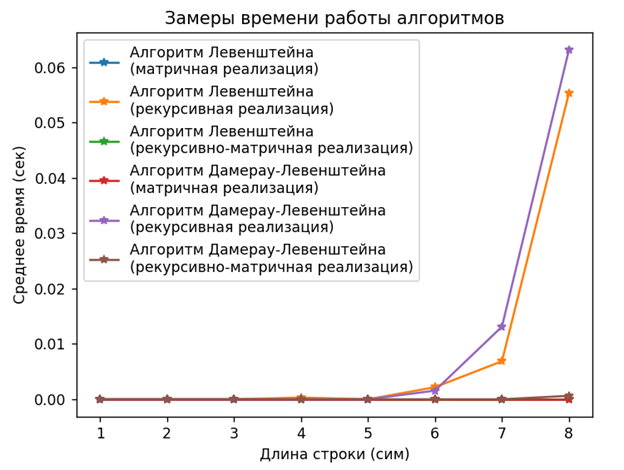
\includegraphics[width=1\textwidth]{img/graph_all.png}
    \caption{График времени работы всех алгоритмов в зависимости от длин строк}
    \label{fig:graph_all} % Метка для ссылки на картинку
\end{figure}

\begin{figure}[H]
    \centering
    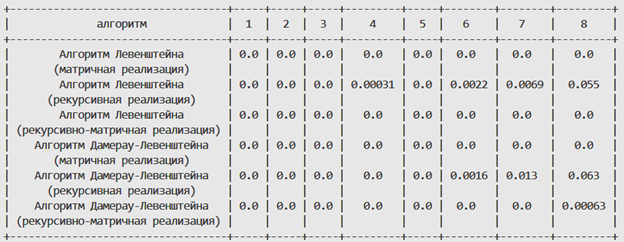
\includegraphics[width=1\textwidth]{img/table_all.png}
    \caption{Таблица времени (сек) работы всех алгоритмов в зависимости от длин строк (сим)}
    \label{fig:table_all}
\end{figure}

\subsection{Сравнение работы матричной, рекурсивной и рекурсивно-матричной реализаций алгоритмов}

\hspace{1.25cm}
Из графиков, приведённых выше, очевидно, что матричная реализация обоих алгоритмов быстро становится эффективнее рекурсивной на много порядков. Это происходит из-за того, что при рекурсии даже на небольшой длине строк происходит много рекурсивных вызовов для подстрок, на что тратится большое количество времени и памяти. В то время как для матричной реализации данные, на основе которых вычисляются следующие значения, хранятся в двух массивах длинной в кратчайшую из двух строк, что экономит как время, так и память. При этом рекурсивно-матричная реализация оказалась почти столь же быстрой, как и матричная благодаря исключению повторных вычислений идентичных веток рекурсии, что в разы сократило количество вычислений.

\subsection{Сравнение работы алгоритмов Левенштейна и Дамерау-Левенштейна (отдельно каждый способ)}

\hspace{1.25cm}
Отдельно было измерено время работы алгоритмов Левенштейна и Дамерау-Левенштейна в их матричных реализациях на большем диапазоне длин рандомно сгенерированных строк (от 25 символов до 125 с шагом 25) по 50 замеров каждая строка, среднее значение было вынесено в таблицу и для наглядности изображено на графике (см. Рис.~\ref{fig:graph_mat} и Рис.~\ref{fig:table_mat}).

\begin{figure}[H]
    \centering
    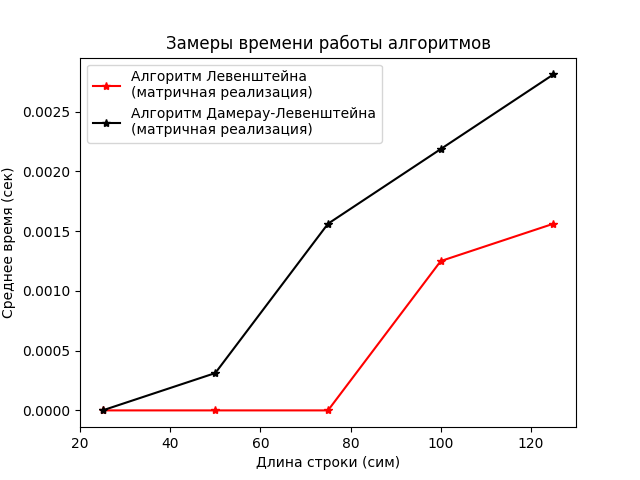
\includegraphics[width=1\textwidth]{img/graph_mat.png}
    \caption{График времени работы матричных реализаций алгоритмов в зависимости от длин строк}
    \label{fig:graph_mat}
\end{figure}

\begin{figure}[H]
    \centering
    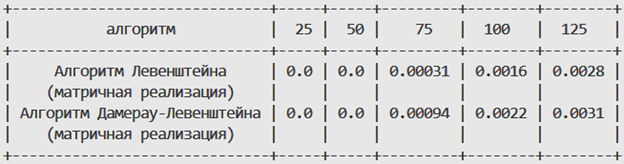
\includegraphics[width=1\textwidth]{img/table_mat.png}
    \caption{Таблица времени (сек) работы матричных реализаций алгоритмов в зависимости от длин строк (сим)}
    \label{fig:table_mat}
\end{figure}

Отдельно было измерено время работы алгоритмов Левенштейна и Дамерау-Левенштейна в их рекурсивных реализациях на малом диапазоне длин рандомно сгенерированных строк (от 1 символа до 9 с шагом 2) по 50 замеров каждая строка, среднее значение было вынесено в таблицу и для наглядности изображено на графике (см. Рис.~\ref{fig:graph_rec} и Рис.~\ref{fig:table_rec}).

\begin{figure}[H]
    \centering
    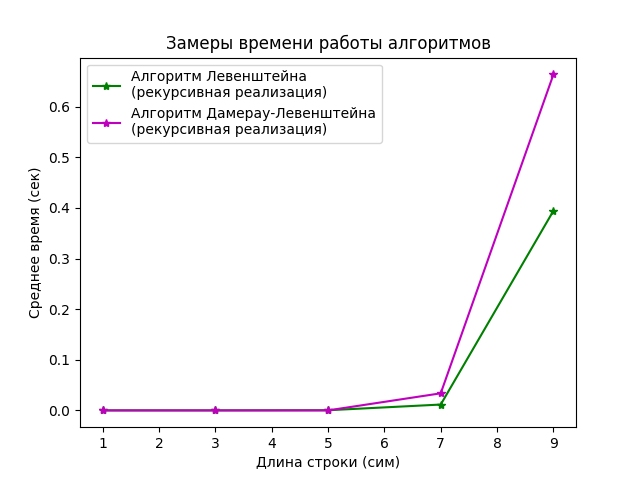
\includegraphics[width=1\textwidth]{img/graph_rec.png}
    \caption{График времени работы рекурсивных реализаций алгоритмов в зависимости от длин строк}
    \label{fig:graph_rec}
\end{figure}

\begin{figure}[H]
    \centering
    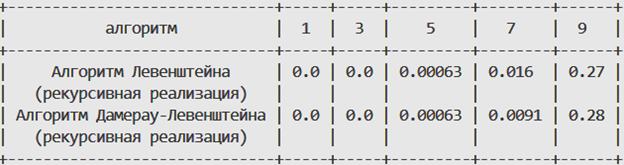
\includegraphics[width=1\textwidth]{img/table_rec.png}
    \caption{Таблица времени (сек) работы рекурсивных реализаций алгоритмов в зависимости от длин строк (сим)}
    \label{fig:table_rec}
\end{figure}

Отдельно было измерено время работы алгоритмов Левенштейна и Дамерау-Левенштейна в их рекурсивно-матричных реализациях на большем диапазоне длин рандомно сгенерированных строк (от 25 символа до 125 с шагом 25) по 50 замеров каждая строка, среднее значение было вынесено в таблицу и для наглядности изображено на графике (см. Рис.~\ref{fig:graph_rec-mat} и Рис.~\ref{fig:table_rec-mat}).

\begin{figure}[H]
    \centering
    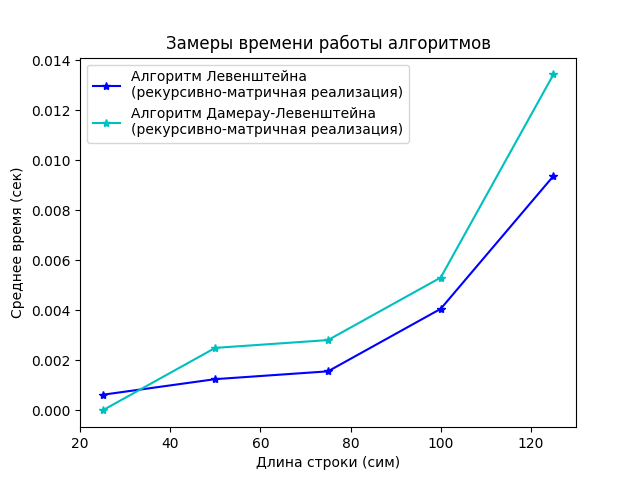
\includegraphics[width=1\textwidth]{img/graph_rec-mat.png}
    \caption{График времени работы рекурсивно-матричных реализаций алгоритмов в зависимости от длин строк}
    \label{fig:graph_rec-mat}
\end{figure}

\begin{figure}[H]
    \centering
    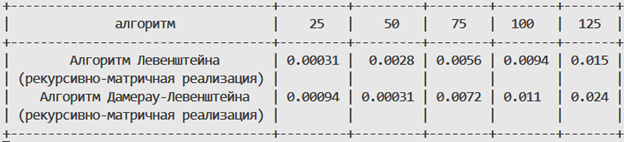
\includegraphics[width=1\textwidth]{img/table_rec-mat.png}
    \caption{Таблица времени (сек) работы рекурсивно-матричных реализаций алгоритмов в зависимости от длин строк (сим)}
    \label{fig:table_rec-mat}
\end{figure}

Видно, что алгоритм Левенштейна оказался немного быстрее алгоритма Дамерау-Левенштейна из-за дополнительной проверки во втором, что компенсируется большим расстоянием в результате первого при наличии перестановок букв в строках.

\subsection{Сравнение работы матричных и рекурсивно-матричных алгоритмов Левенштейна и Дамерау-Левенштейна}

\hspace{1.25cm}
Так как на общем графике матричный и рекурсивно-матричный алгоритмы были очень близки по скорости, были проведены отдельные замеры (на 5-и точках с длиной строк от 25 до 125 символов с шагом 25 по 50 запусков), среднее значение было вынесено в таблицу и для наглядности изображено на графике (см. Рис.~\ref{fig:graph_mat_rec-mat} и Рис.~\ref{fig:table_mat_rec-mat}).

\begin{figure}[H]
    \centering
    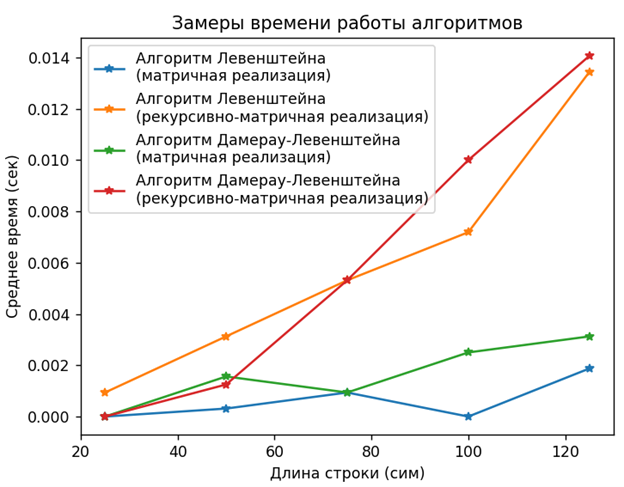
\includegraphics[width=1\textwidth]{img/graph_mat_rec-mat.png}
    \caption{График времени работы матричных и рекурсивно-матричных реализаций алгоритмов в зависимости от длин строк}
    \label{fig:graph_mat_rec-mat}
\end{figure}

\begin{figure}[H]
    \centering
    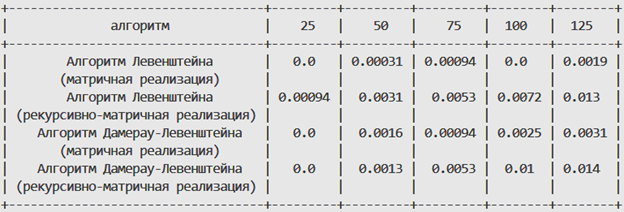
\includegraphics[width=1\textwidth]{img/table_mat_rec-mat.png}
    \caption{Таблица времени (сек) работы матричных и рекурсивно-матричных реализаций алгоритмов в зависимости от длин строк (сим)}
    \label{fig:table_mat_rec-mat}
\end{figure}

По результатам приведённых графиков видно, что и в алгоритме Левенштейна и Дамерау-Левенштейна рекурсивно-матричный метод работает дольше матричного. Это объясняется затратами на вызов функции при рекурсии и на дополнительные проверки является ли искомое значение уже посчитанным. На небольших длинах строк разница в скорости работы алгоритмов отличается несущественно, однако с увеличением данных растёт и разница во времени.

\subsection*{Вывод}

\hspace{1.25cm}
По проведённым исследованиям была выявлена большая скорость работы алгоритма Левенштейна над алгоритмом Дамерау-Левенштейна за счёт уменьшения числа проверок, что, однако, даёт иной результат при наличии возможности перестановок символов в строках. При этом матричный вариант выигрывает по скорости в обоих алгоритмах, на втором месте оказался рекурсивно-матричный метод, который делает меньше рекурсивных вызовов, чем рекурсивный метод, и исключает повторные вычисления идентичных веток, так как при вызове каждой новой функции в этом методе передаётся в качестве аргумента ссылка на матрицу, которая хранит уже посчитанные значения, но на эту матрицу также необходима память, а проверки на уже вычисленные значения не всегда приносят положительный результат и занимают время.

\newpage